\title{A Unifying Language for Database And User Interface Development}
\author{Alexander Burger}
% Use \authorrunning{Short Title} for an abbreviated version of
% your contribution title if the original one is too long
\institute{\texttt{abu@software-lab.de}}
%
% Use the package "url.sty" to avoid
% problems with special characters
% used in your e-mail or web address
%


\maketitle

% \section{A Unifying Language for Database And User Interface Development}
% \label{sec:unifying-language}


% \subsection{A Unifying Language for Database And User Interface Development}
% \label{sec-2-2}
% \label{unifying-language}


% 2002-06-16 (c) Software Lab. Alexander Burger (originally published
% \href{http://www.software-lab.de/dbui.html}{here}). 


\begin{abstract}
A language framework is presented which closes the semantic gap between
database, application logic, and user interface. We introduce the
concepts of Prefix Classes and Relation Maintenance Daemon Objects to
suggest a unified development style reducing software development time
and cost.
\end{abstract}

 
\section{Introduction}
\label{sec:ul-intro}

Ever since computers were used in commercial applications, there was a
growing demand to reduce software development time and cost.

Business models are quite different from each other. Off-the-shelf
software usually does not fit the individual needs for enterprise
workflow data processing, real world modeling, and multimedia
applications. For that reason, many companies are forced to develop
their own solutions. Software is a significant cost factor.

Due to the competitive nature of business, the redundancy inherent in
such individual developments can hardly be avoided. Concerning the
development costs, however, there seems to be a lot of room for
improvements.

Typically, these projects implement some kind of database and a set of
application programs. The task of these programs is to manipulate the
data in the database, implement the general application logic, and
provide for some kind of user interface.

We observe a large semantic gap between the database structure, and the
application logic with its user interface. The current standard database
language is \texttt{SQL}, which operates on the table level, while
general-purpose programming languages like \texttt{Cobol}, \texttt{C/C++} or \texttt{Java}
are used to implement the application logic and user interface.

In numerous attempts to remedy the situation, object-oriented paradigms
are applied to both ends, by extending the relational database to
object-oriented databases, and by building user interface frameworks in
object-oriented languages.

There's no doubt that object-oriented databases provide for more
intuitivity and productivity, and modern graphical user interfaces (GUI)
cannot not be imagined without those frameworks.

But the semantic gap does not appear to diminish significantly.
Databases and user interfaces are separate worlds: Existing class
libraries are concerned about visual effects and event handling, but not
about application logic and database maintenance. It is the programmer's
responsibility to write glue code that displays data in corresponding
GUI fields, detects modifications by the user, validates them, writes
changes back to the database, and does other housekeeping.

This paper introduces a language and programming environment that closes
the semantic gap, by unifying database and user interface into a single
application server framework.

 
\section{Traditional DB and GUI Development}
\label{sec:ul-trad-db-gui-devel}

The mainstream database format today is still the relational model,
which packs the application data into two-dimensional tables, and relies
on the application program logic to correctly access these data and to
maintain their integrity via proper \texttt{SQL} statements.

A single data record on the application level (like, for example, a
customer or an article) - which is presented to the user within a single
GUI window - is usually spread out over several tables in the database.

The application program has to \texttt{select} these data, explicitly supplying
knowledge about the relations between the tables, the data types and
sizes, then have them copied to variables in the application scope, and
move them to the GUI window. (Note: There are tendencies to ``hide'' this
code into the methods of an object-relational database. This serves well
for better structuring the application program design, but does not
decrease the actual amount of programming work. The correct
\texttt{select}-statements still have to be written, and a change in the
relations or table structures may require individual modifications.)

The GUI components have access to these variables in the application
scope; they are notified after a successful \texttt{select} to display these
data.

Now comes the most tedious part. The user interface cannot simply wait
until a user has done all his changes to the data record and hits some
``submit''-button. It is necessary to provide immediate feedback on field
entry, field exit, and often on every key stroke or mouse click.
Depending on the context and the internal state of the application,
individual GUI components or program features have to be enabled or
disabled.

When the focus leaves a GUI component, its data have to be validated
(possibly displaying error messages to the user), certain side-effects
carried out (which might influence other GUI components), and
modifications written to the database. A simple change in a single text
field can cause an \texttt{update} to several database tables.

All these things involve \texttt{SQL} statements which again must contain
extensive knowledge about the database structure. And they cannot easily
be abstracted into reusable DB- or GUI-classes, because the requirements
tend to differ for each view on the data record and each combination of
GUI components. Thus, they have to be written individually for each GUI
window.

 
\section{A Unified Approach}
\label{sec:ul-unified-approach}


We use the \texttt{PicoLisp} interpreter to build a vertical, unified solution
to these problems. It allows to describe a direct mapping between
application structures and database objects, so that the underlying
machine can handle most of the above issues automatically.

The solution is ``vertical'', because it extends from the virtual machine
level up into the application and GUI levels. And it ``unifies'', in a
consistent way, the \texttt{Lisp} interpreter with

\begin{itemize}
\item a flexible object architecture
\item an object-oriented database
\item relation maintenance daemon objects
\item a Prolog-equivalent query language. (Note: ``Unified'' is also a pun
   here, as it is fundamental to the Prolog terminology.)
\item and a user interface strategy
\end{itemize}

by using the same syntax and philosophy all along the way. We will
describe its details in the following sections, and give some practical
examples.

It turned out that certain requirements for the virtual machine are not
met by existing languages like \texttt{C++} and \texttt{Java}. These requirements
include dynamic I/O of persistent objects, and a garbage collector
handling these objects accordingly.

\texttt{PicoLisp} was chosen as the base language, because its interpreter is
simple and completely written in \texttt{C}. This makes it easy to incorporate
the necessary extensions to the virtual machine. Besides this, two other
features (of \texttt{Lisp} in general)

\begin{itemize}
\item dynamic data types and structures
\item and formal equivalence of code and data
\end{itemize}

are considered essential. They are both needed for the intended
descriptive syntax of the resulting application development system.

 
\subsection{Object Architecture}
\label{sec:ul-obj-arch}


\texttt{PicoLisp} employs a very simple object architecture. It uses
\emph{symbols} for the implementation of both classes and objects.
There are many ways to implement symbols in \texttt{Lisp}~\cite{allen};
in \texttt{PicoLisp} each symbol has a value cell, a property list,
and a name.

For a symbol representing an \emph{object}, the value cell holds a list of
the object's classes, the property list holds the object's attributes
(instance variables), and the name is usually empty (anonymous symbol).

For a symbol representing a \emph{class}, the value cell holds an association
list with the class' methods, concatenated with a list of the class'
superclasses, the property list may hold some class attribues (class
variables), and the symbol's name is the name of the class.

When a \emph{message} (also a symbol) is sent to an object, that object's
list of classes - and recursively those classes' superclasses - is
searched from left to right (in a depth-first manner) for that message,
and the corresponding \emph{method} body is executed. (In effect, this is a
multiple-inheritance late-binding strategy.)

In that way, a class \texttt{+MyCls} can be defined to inherit from
three classes \texttt{+Cls1}, \texttt{+Cls2} and \texttt{+Cls3} (by
convention, class names start with a `\texttt{+}'):


\begin{wideverbatim}
(class +MyCls +Cls1 +Cls2 +Cls3)
\end{wideverbatim}

Then, an object can be created with


\begin{wideverbatim}
(new '(+MyCls))
\end{wideverbatim}

or another object with equivalent behavior:


\begin{wideverbatim}
(new '(+Cls1 +Cls2 +Cls3))
\end{wideverbatim}

In both cases the resulting objects will inherit method definitions from
\texttt{+Cls1}, \texttt{+Cls2} and \texttt{+Cls3}. Because of the depth-first and
left-to-right search order, however, methods in the class hierarchy of
\texttt{+Cls1} will override methods with the same name anywhere in the class
hierarchies of \texttt{+Cls2} and \texttt{+Cls3}.

This is a ``horizontal'' inheritance, as opposed to - and in addition to -
the normal ``vertical'' inheritance. \texttt{+Cls1} and \texttt{+Cls2} can surgically
alter the behavior of \texttt{+Cls3}, in a very fine-grained manner. Thus - as
\texttt{+Cls3} will typically define the general behavior - \texttt{+Cls1} and \texttt{+Cls2}
are called \emph{Prefix Classes} of \texttt{+Cls3}.

This object architecture is used throughout the whole system, including
the DB and GUI. And prefix classes are an essential part of it: The
expressive power of \texttt{Lisp}'s equivalence of code and data is augmented
in combination with prefix classes.

 
\subsection{Database}
\label{sec:ul-databast}


The \texttt{PicoLisp} database is built upon that object architecture.

On the lowest level, a database is a collection of persistent objects.
\texttt{PicoLisp} supports persistent symbols, called \emph{external} symbols, as a
first-class data type. These symbols are known to - and handled in
special ways by - the interpreter.

External symbols are stored in a file, in linked blocks of fixed size,
where each symbols's starting block address is computable from the
symbols's name.

A read or write access to an external symbol's value or properties
causes that symbol to be automatically fetched from the database file.
At the end of any transaction, modified symbols are written back
(\texttt{commit}) or reverted (\texttt{rollback}). The garbage collector knows about
the state of external symbols, and purges currently unused symbols from
memory (Note: These symbols are only temporarily removed from memory,
not from the database. The latter is done separately by a DB-level
garbage collector.).

On the higher levels, these external symbols are organized into class
hierarchies, reflecting the application's organizational structures.

As opposed to simple two-dimensional tables, they form arbitrary data
structures like lists, stacks, trees and graphs.

The connections (relations) between objects in the database are not
established by index lookup, but by explicit inclusion. That is, an
object referring to another object can explicitly hold (i.e. contain a
pointer to) that object, and can get access to it very rapidly. There is
no explicit \texttt{select} operation, everything is simply available when it
is needed.

 
\subsection{Relation Daemons}
\label{sec:ul-rel-daemons}


Generally, instances of persistent database objects are called
``Entities''. In our system, there is an additional separate class
hierarchy of ``Relations'': Instances of these classes we call ``relation
maintenance daemon objects''.

Relation daemons are a kind of \emph{metadata}, controlling the interactions
between entities, and maintaining database integrity. They are the
concrete realization of an abstract Entity/Relationship.

Like other classes, relation classes can be extended and refined, and in
combination with proper prefix classes a fine-grained description of the
application's structure can be produced.

Besides some primitive relation classes, like \texttt{+Number}, \texttt{+String} or
\texttt{+Date}, there are

\begin{itemize}
\item relations between entities, like \texttt{+Link} (uni-directional link),
   \texttt{+Joint} (bi-directional link) or \texttt{+Hook} (object-local index root)
\item relations that bundle other relations into a single unit (\texttt{+Bag})
\item a \texttt{+List} prefix class
\item prefix classes that maintain index trees, like \texttt{+Key} (unique index),
   \texttt{+Ref} (non-unique index) or \texttt{+Idx} (full text index)
 \item prefix classes which in turn modify index class behavior, like
   \texttt{+Sn} (soundex algorithm for tolerant searches)~\cite{knuth}
\item a \texttt{+Need} prefix class, for existence checks
\item a \texttt{+Dep} prefix class controlling dependencies between other
   relations
\end{itemize}

A defining function \texttt{rel} is provided, which is used in the context of
an entity class to assign relation daemon objects to that class:


\begin{wideverbatim}
(rel attr (+Cls ..) Arg ..)
\end{wideverbatim}

\texttt{rel} is called with an attribute name \texttt{attr}, a list of relation
classes \texttt{(+Cls ..)} and - depending on these classes - other optional
arguments. Basically, this function simply does a


\begin{wideverbatim}
(new '(+Cls ..) Arg ..)
\end{wideverbatim}

and assigns the resulting daemon object to the \texttt{attr}-property of the
current entity class.

 
\subsubsection{Relation Prefix Usage}
\label{sec:ul-relat-pref-usage}
For example, a simple entity ``Person'' can be defined, having just a
``name'' attribute:

\begin{wideverbatim}
(class +Person +Entity) # class '+Person'
(rel name (+String))    # relation 'name'
\end{wideverbatim}

If the \texttt{name} relation needs a unique index, it is written as:


\begin{wideverbatim}
(rel name (+Key +String))
\end{wideverbatim}

And - for an extended example of prefix classes - if \texttt{name} should be a
mandatory list of names, each with an index using the soundex algorithm:


\begin{wideverbatim}
(rel name (+Need +List +Sn +Idx +String))
\end{wideverbatim}

This demonstrates the power of combined prefix classes, which allow to
define complex object behavior ``on the fly'', without the need to leave
the current programming focus. This is even more important in user
interface programming (see section~\vref{sec:ul-gui-integration}).


\subsubsection{Entity Linkage}
\label{sec:ul-entity-linkage}

A uni-directional link to another entity might be, for example, the
person's address:


\begin{wideverbatim}
(rel adr (+Link) (+Address))
\end{wideverbatim}

This assumes that some entity class \texttt{+Address} is defined:


\begin{wideverbatim}
(class +Address +Entity)
\end{wideverbatim}

In reality, the relation will probably be bi-directional, with several
persons living at some address:


\begin{wideverbatim}
(class +Person +Entity)
(rel adr (+Joint) prs (+Address))

(class +Address +Entity)
(rel prs (+List +Joint) adr (+Person))
\end{wideverbatim}

This says: The \texttt{adr}-attribute of \texttt{+Person} (a \texttt{+Joint}) is an address
(connected to the \texttt{prs}-attribute of \texttt{+Address}), while the
\texttt{prs}-attribute of \texttt{+Address} (a \texttt{+List +Joint}) is a list of persons
(connected to the \texttt{adr}-attribute of each person).

So, when a person's \texttt{adr} is assigned to some address, the \texttt{+Joint}
relation daemon will take care of updating the list of persons in that
address, and vice versa.

\subsection{Query Language}
\label{sec:ul-query-language}


For extensive searches in the database, as they are needed for reports
or user-specified queries, a \texttt{Prolog} engine was incorporated into
\texttt{PicoLisp}. \texttt{Prolog} is similar to \texttt{SQL}, due to its declarative nature,
but much more powerful because of its rule-deriving and backtracking
capabilities.

\texttt{Prolog} is easy to implement in \texttt{Lisp}~\cite{campbell}.
We extended the basic inference machine to iterate also through facts
in the database, and the basic search/backtracking algorithm to a
self-optimizing parallel search through multiple index trees.

The details of the query language are beyond the scope of this paper. It
is mentioned here because our production system would be incomplete
without it.

 
\subsection{GUI Integration}
\label{sec:ul-gui-integration}

The connection between database objects and GUI components is
established with only two prefix classes: \texttt{+E/R} and \texttt{+Obj}.

Normally, GUI components are created at runtime with the \texttt{gui} function,
e.g.


\begin{wideverbatim}
(gui '(+TextField) "Text" 8)
(gui '(+NumField) "Number" 8)
\end{wideverbatim}

for a text field and a numeric field, each 8 characters wide.
 
\subsubsection{\texttt{+E/R} (Entity/Relation)}
\label{sec:ul-entity-relation}

The \texttt{+E/R} prefix connects the GUI field with a given relation of an
entity:

\begin{wideverbatim}
(gui '(+E/R +NumField) '(n . Obj) "Number" 8)
\end{wideverbatim}

The specification \texttt{(n . Obj)} is passed as an additional argument. It
indicates that this numeric field is ``connected'' to the \texttt{n}-property of
the database object \texttt{Obj}.

Nothing else has to be done by the programmer. The field will
automatically display the value of \texttt{n} from the database, and
modifications entered by the user into this field will be written
automatically to the database value of \texttt{n}, in the object \texttt{Obj}.

\subsubsection{\texttt{+Obj} (Object)}
\label{sec:ul-object}

The \texttt{+Obj} prefix extends the GUI field types, from primitives like
numbers or strings, to database objects.

That is, a GUI field can ``contain'' a database object, just like a text
field contains a string, and a numeric field contains a number. An
object can be ``set'' into (assigned to) the field, and retrieving the
value of the field will result in that object.

The field cannot, of course, directly display the complete database
object. But it can show a typical attribute of that object, e.g. the
object's name in a text field, or the object's ID number in a numeric
field:

\begin{wideverbatim}
(gui '(+Obj +NumField) '(id +Cls) "ID" 8)
\end{wideverbatim}

The \texttt{+Obj} prefix extends the capabilities of the basic field type (here
a \texttt{+NumField}), in such a way that

\begin{itemize}
\item a proper attribute value is displayed when an object is assigned to
   the field
\item the field is set to the corresponding object when a legal attribute
   value is entered
\item the field performs keyboard auto-expansion to legal attribute values
   directly out of the database
\item the field can display a choice list for matching attribute values
\item the fields opens an editor for that object when it is double-clicked
   (Hyper-Link)
\end{itemize}

As a consequence, when \texttt{+E/R} and \texttt{+Obj} are combined


\begin{wideverbatim}
(gui '(+E/R +Obj +NumField) '(x . Obj) '(id +Cls) "Number" 8)
\end{wideverbatim}

they effectively establish the GUI for an entity linkage (\texttt{+Link},
\texttt{+Joint} etc.), as described in section~\vref{sec:ul-entity-linkage}. 

 
\section{An Example}
\label{sec:an-example}

Putting it all together, the total effect of the described concepts can
best be explained with the help of a detailed and complete example.

Assuming a simple family database, we represent a network of family
relationships. For each person, we have attribues for name, sex, date of
birth, and we want to have links to father, mother, husband/wife and
children.

For a better understanding, we first present the traditional, relational
representation (Note that we have to introduce a unique ID number for
each record. Also, in such a tabular representation, it is more
convenient to store the ID of father and mother (instead of the
children).):


\begin{center}
\begin{tabular}{rlllrrr}
 ID  &  nm       &  sex  &  dat        &  mate  &  pa  &  ma  \\
\hline
  1  &  John     &  M    &  22jan1954  &     2  &      &      \\
  2  &  Mary     &  F    &  01feb1958  &     1  &      &      \\
  3  &  Thomas   &  M    &  26jan1988  &        &   1  &   2  \\
  4  &  Claudia  &  F    &  15jul1989  &        &   1  &   2  \\
  5  &  Michael  &  M    &  03jan1992  &        &   1  &   2  \\
\end{tabular}
\end{center}


When viewing the these family members as a graph, we get the following
object structure:

\begin{figure}[H]
  \centering
  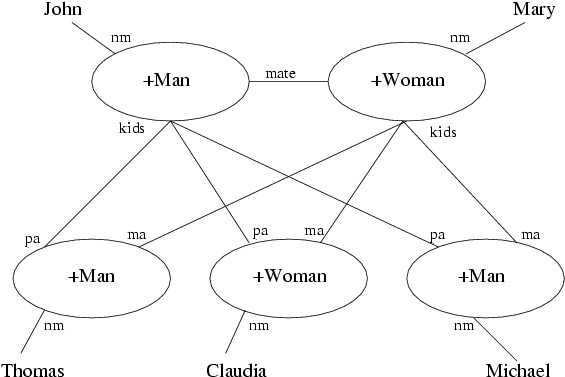
\includegraphics[scale=.5]{graphics/xmplObj.jpg}
  \caption{Family Members}
  \label{fig:family-members}
\end{figure}

In the figure, we omitted the date of birth attribute.

The bi-directional relations, connecting the parents to the children and
to each other, lend themselves to the \texttt{+Joint} entity linkage, resulting
in the following definition for a person:


\begin{wideverbatim}
(class +Person +Entity)
(rel nm   (+Key +String))          # Name
(rel pa   (+Joint) kids (+Man))    # Father
(rel ma   (+Joint) kids (+Woman))  # Mother
(rel mate (+Joint) mate (+Person)) # Partner
(rel dat  (+Date))                 # born
\end{wideverbatim}

From this base class, we can derive two classes \texttt{+Man} and \texttt{+Woman}:


\begin{wideverbatim}
(class +Man +Person)
(rel kids (+List +Joint) pa (+Person))

(class +Woman +Person)
(rel kids (+List +Joint) ma (+Person))
\end{wideverbatim}

To produce a corresponding GUI


\begin{figure}[H]
  \centering
  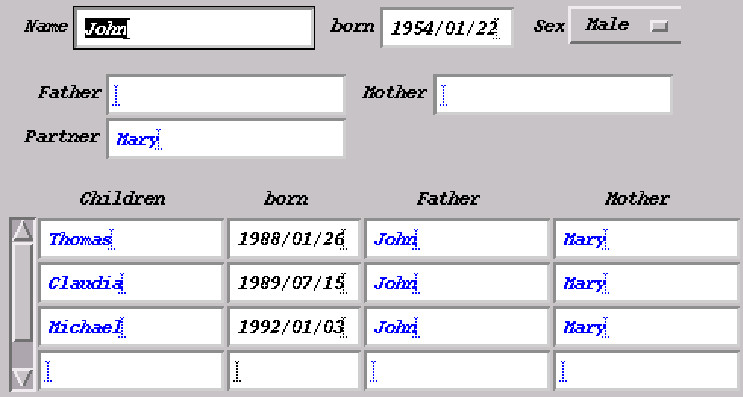
\includegraphics[scale=.5]{graphics/xmplGui.jpg}
  \caption{GUI}
  \label{fig:family-gui}
\end{figure}


allowing to view and edit the family members in the database, the
following code is sufficient:


\begin{wideverbatim}
(row
   (gui '(+E/R +TextField) '(nm : home obj) "Name" 20)
   (gui '(+E/R +DateField) '(dat : home obj) "born" 10)
   (gui '(+ClassField)
      '(: home obj) "Sex"
      '(("Male" +Man) ("Female" +Woman)) ) )
(----)
(row
   (gui '(+E/R +Obj +TextField)
      '(pa : home obj) '(nm +Man)
      "Father" 20 )
   (gui '(+E/R +Obj +TextField)
      '(ma : home obj) '(nm +Woman)
      "Mother" 20 ) )
(gui '(+E/R +Obj +TextField)
   '(mate : home obj) '(nm +Person)
   "Partner" 20 )
(---- T)

\end{wideverbatim}

\begin{wideverbatim}

(gui '(+E/R +Chart)
   '(kids : home obj)
   4 '("Children" "born" "Father" "Mother")
   (quote
      (gui '(+Obj +TextField) '(nm +Person) "" 15)
      (gui '(+Skip +Lock +DateField) "" 10)
      (gui '(+ObjView +TextField) '(: nm) "" 15)
      (gui '(+ObjView +TextField) '(: nm) "" 15) ) )
\end{wideverbatim}

The above block of code will produce exactly the layout and
functionality of the example GUI display. Without explaining all details
here, suffice it to say that the \texttt{row} function arranges the components
horizontally (while otherwise the default is vertically), \texttt{(-{}-{}-{}-)}
groups components into separate panels, and a \texttt{+Chart} creates an array
of its argument components.

The point is that this is the \emph{complete program}, not just some
important details. It specifies the whole database and GUI application.

 
\section{Discussion}
\label{sec:ul-discussion}

The previous sections and the example show that application programming
does not need to involve any concerns about database access (select,
insert, update etc.) and database integrity maintenance.

The advantages are derived from the use of prefix classes and relation
daemons. They allow to specify the complete program behavior and
appearance in a single place of definition, and in a very concise form.
Typically, the names of prefix classes are simply chained together, and
intermix freely with \texttt{Lisp}'s formal indifference of code and data.

This removes the need of maintaining separate resource files, class and
data declarations, and program code.

 
\section{Conclusion}
\label{sec:ul-conclusion}

Achieving low program development costs is an old claim. It has been
stated for manyfold methodologies and paradigms.

The system described in this paper has proven its practical value in
commercial applications during several years. Among them are sales,
accounting, report, and logistics applications. Research projects
include graphics/animation and speech synthesis systems.

This shows that it is possible to employ the concepts of prefix classes
and relation maintenance daemons successfully to commercial application
development.

We observed a significant decrease in program development time. What
used to be the major part of a project's development effort showed to
reduce to about 5 percent.

 
\section{Download}
\label{sec:ul-download}

The \texttt{PicoLisp} system can be downloaded from the
\href{http://www.software-lab.de/down.html}{PicoLisp Download}
Page~\cite{down2}.

\begin{thebibliography}{[9]}

\bibitem{allen} John Allen: ``Anatomy of Lisp'', McGraw-Hill, 1978

\bibitem{knuth} Donald E. Knuth: ``The Art of Computer Programming'',
  Vol.3, Addison-Vesley, 1973, p. 392

\bibitem{campbell}J. A. Campbell: Implementations of Prolog, Ellis Horwood Limited, 1984

\bibitem{down2} Pico Lisp Download, http://www.software-lab.de/down.html

\end{thebibliography}


